\hsection{Floating Point Numbers}%
%
In the previous section, we have discussed integers in \python.
One of the very nice features of the \python~3 language is that integers can basically become arbitrarily large.
There is only the single type \pythonil{int} and it can store any integer value, as long as the memory of our computer is large enough.%
%
\begin{sloppypar}%
In an ideal world, we would have a similar feature also for fractional numbers.
However, such a thing cannot be practically implemented.
You will certainly remember the numbers $\pi\approx3.141\decSep592\decSep653\decSep590\dots$ and $e\approx2.718\decSep281\decSep828\decSep459\dots$ from highschool maths.
They are transcendental~\cite{N1939TTOP,APM1991TOEAP,F2011TTOEAP}, i.e., their fractional digits never end and nobody has yet detected an orderly pattern in them.
Since these numbers are \inQuotes{infinitely long,} we would require infinitely much memory to store them \emph{if} we wanted to represent them \emph{exactly}.
So we don't and neither does \python.
We cannot really represent the real numbers~\realNumbers\ exactly in the memory of our computers.%
\end{sloppypar}%
%
\hsection{How Floating Point Numbers Work}%
\label{sec:howFloatingPointNumbersWork}%
%
\begin{figure}%
\centering%
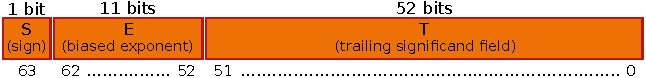
\includegraphics[width=0.7\linewidth]{\currentDir/floatIEEEStructure}%
\caption{The structure of an 64~bit / double precision IEEE~Standard 754 floating point number~\cite{IEEE2019ISFFPA,H1997IS7FPN}.}%
\label{fig:floatIEEEStructure}%
\end{figure}%
%
With \pythonil{float}, \python\ offers us one type for fractional numbers.
This datatype represents numbers usually in the same format as \pythonil{double}s in the \pgls{C}~programming language~\cite{PSF2024NTIFC}, which, in turn, internally have a 64~bit IEEE~Standard 754 floating point number layout~\cite{IEEE2019ISFFPA,H1997IS7FPN}.

The idea behind this standard is to represent both very large numbers, like~$10^{300}$ and very small numbers, like~$10^{-300}$.
In order to achieve this, the 64~bits are divided into three pieces, as illustrated in \cref{fig:floatIEEEStructure}.

The first part, the so-called \pgls{significand} or \pgls{mantissa}, consists of 52~bits, represents the digits of the number.
52~bits can represent $52\log_2 10\approx 15$~decimal digits, meaning that we can represent numbers to a precision of about 15~digits.
If we would just use 52~bits, then this would limit us to represent numbers maybe from~$0$ to~$2^{52}-1$ at a resolution of~$1$.
Of course, we could also choose some other resolution, say~$0.001$.
In this case, we could represent numbers from~$0$ to $0.001*(2^{52}-1)$ and the smallest non-zero number would be~$0.001$ instead of~$1$.
Whatever fixed resolution we would choose, it would be good in some cases and bad in others.

Therefore, the second part of the 64~bit floating point number representation comes into play:
The 11~bits of the \pgls{exponent} represent a power of~2 which is multiplied to the \pgls{significand} to get the actual number.
In order to allow us to have both small and large numbers, this value must be able represent positive and negative exponents.
Therefore, the stored value of the \pgls{exponent} is taken and a \pgls{bias} of~1023 is subtracted.
Thus, a stored value of 2000 in the exponent fields leads to an actual exponent of $1050-1023=27$, which would mean that the \pgls{significand} is multiplied with~$2^{27}$, i.e., $134\decSep217\decSep728$.%
%
\begin{sloppypar}%
Finally, the \pgls{signBit} in the floating point number dataformat indicates whether the number is positive or negative.
Together, this allows us to represent numbers from $2.225\decSep073\decSep858\decSep507\decSep201\decSep4*10^{-308}$ to $1.797\decSep693\decSep134\decSep8623\decSep157*10^{308}$ with a resolution of approximately 15~digits.
Of course, the same range also applies to negative numbers and $0$~can be represented as well.
Indeed, there are even special floating point values for infinity and errors.
But more about this later.%
\end{sloppypar}%
%
Luckily, you will never really need to know these exact information.
The important thing to remember is:
Floating point numbers can represent a wide range of different values.
Their range is large but still limited.
They can represent integers and fractions.
However, their accuracy is always limited to about 15~digits.
In other words, regardless whether your \pythonil{float} stores a very large or a very small number, you can have at most 15~digits of precision.
For example, adding~1 to~$10^{16}$ would still yield~$10^{16}$, because only 15~digits are \inQuotes{stored} and the~1 will just \inQuotes{fall off.}
You cannot represent numbers arbitrarily precisely.%
\endhsection%
%
\endhsection%
%
